\subsection{Comparing provenances through time}

To show how the DS based on different provenances may actually differ in their behavior, let us consider Figure \ref{fig:comparison}.

\begin{figure}[]
  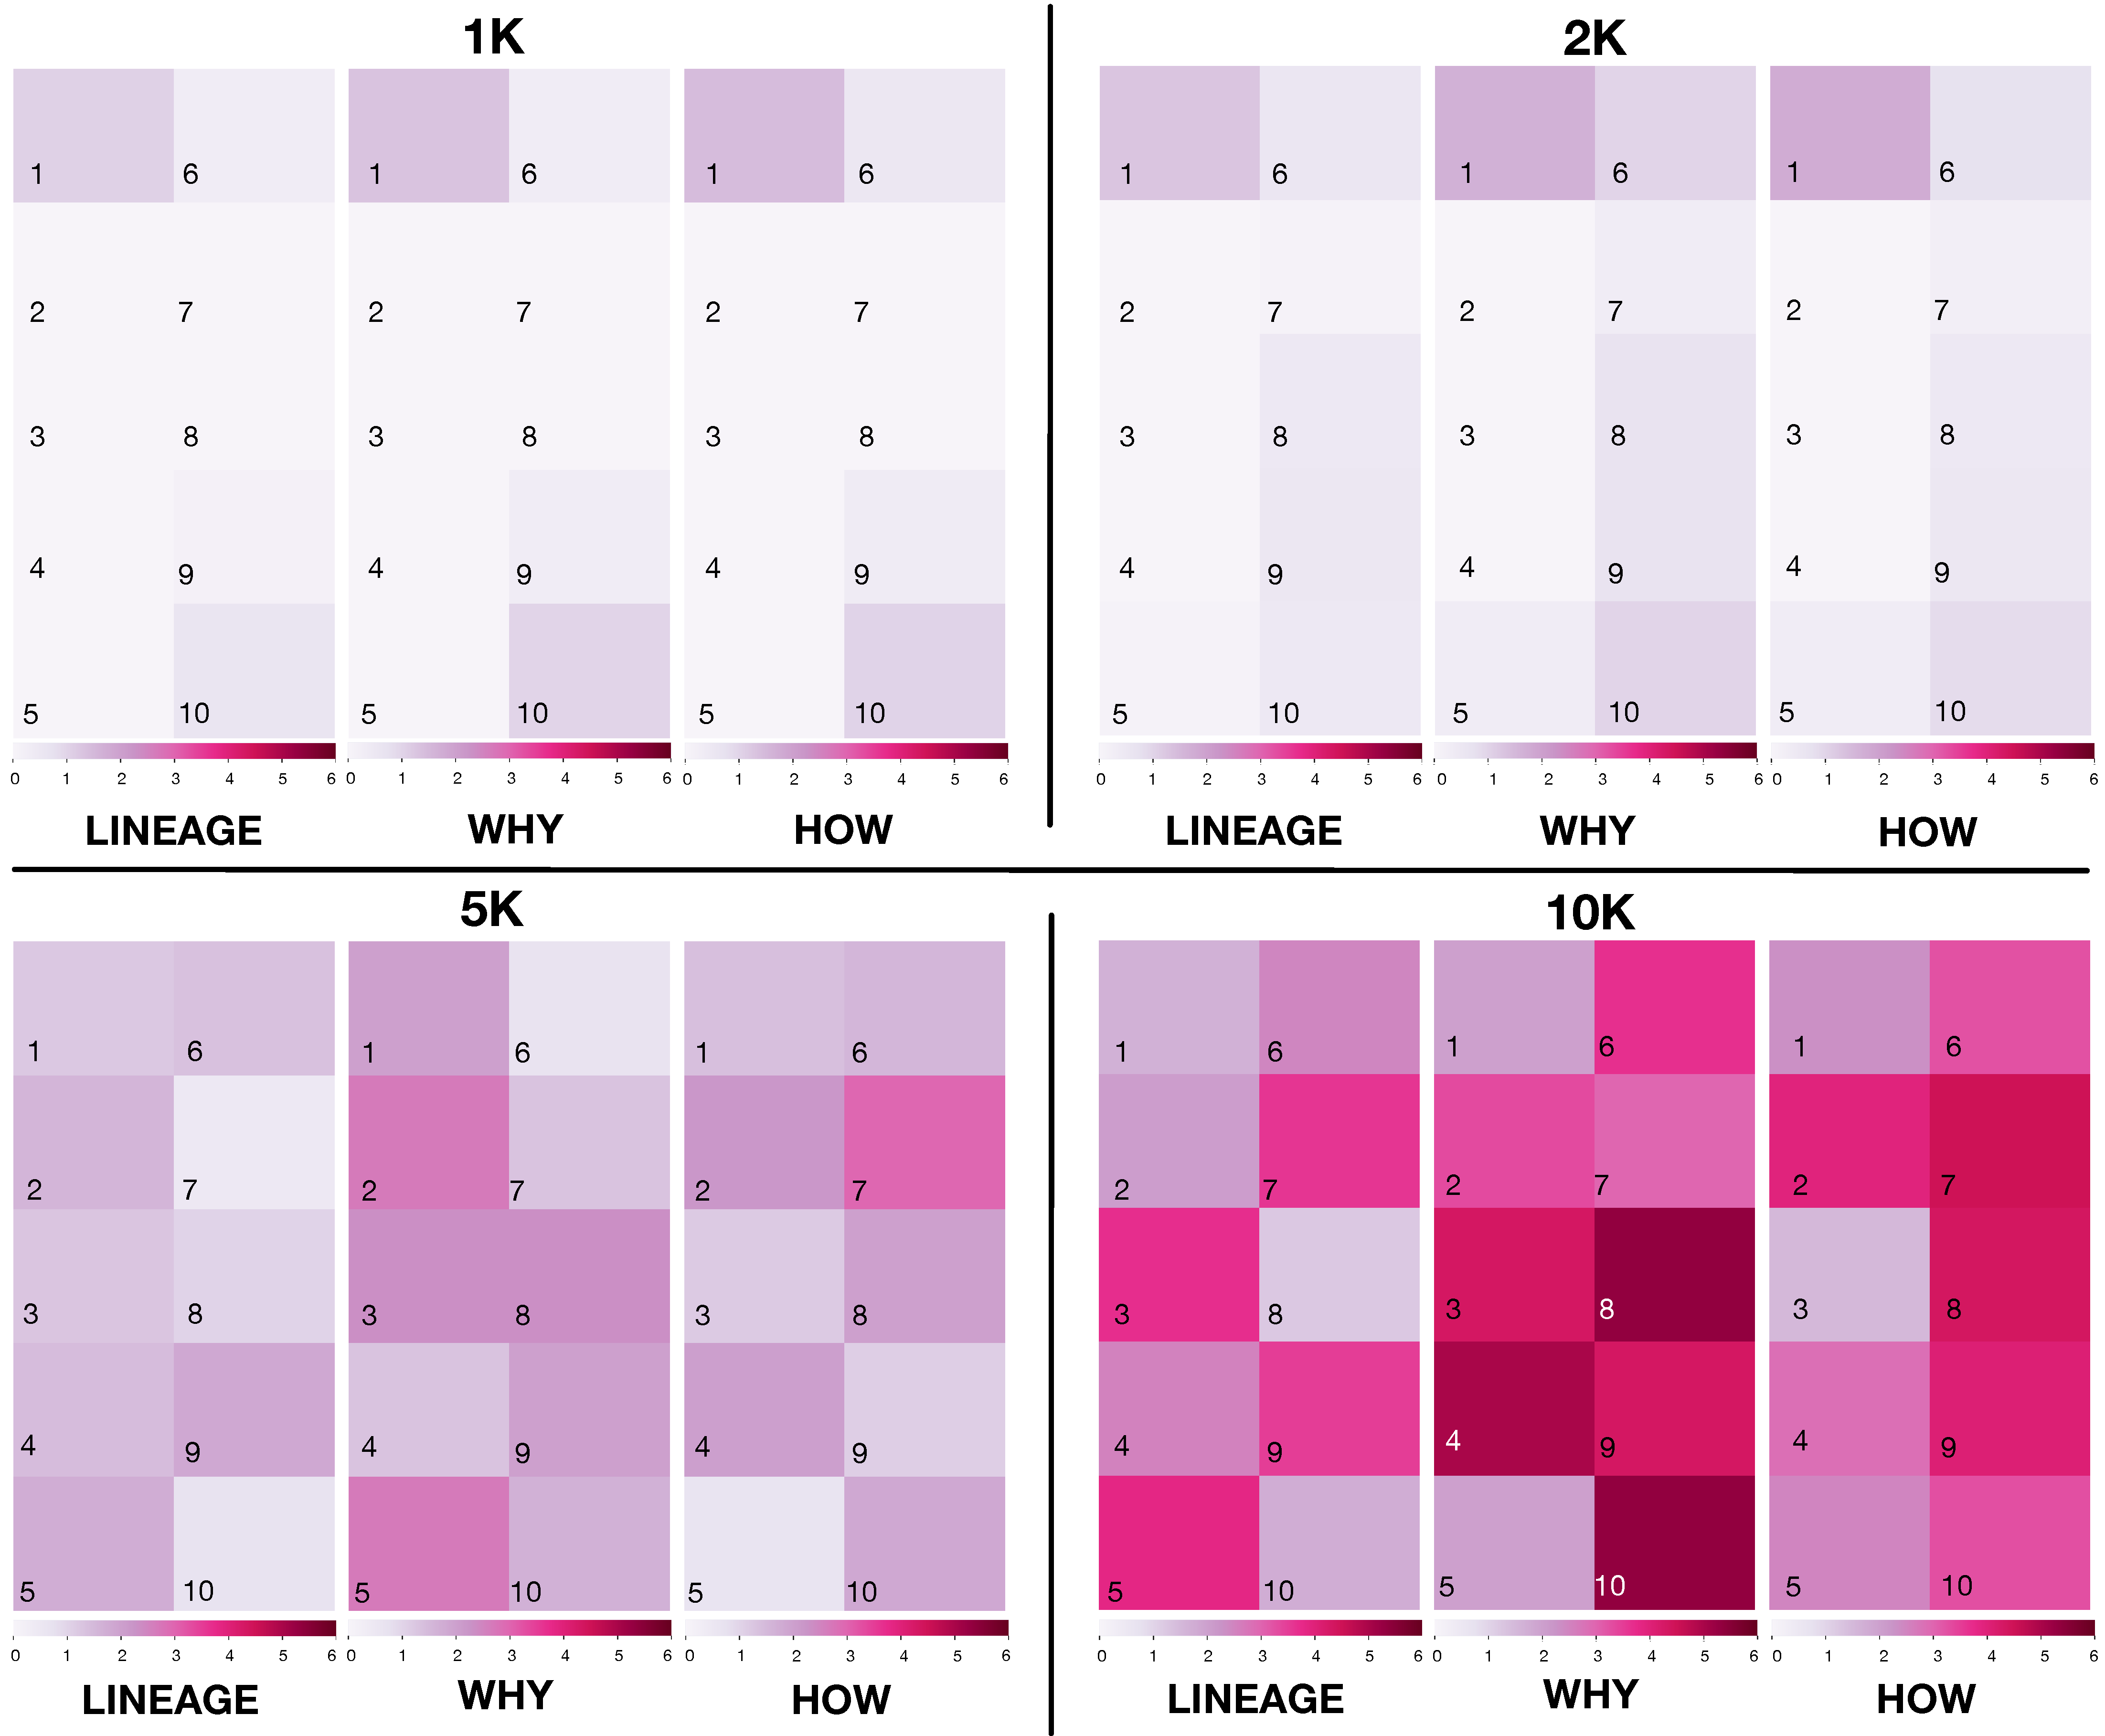
\includegraphics[width=\textwidth]{figures/comparison}
  \caption{Comparison of the distribution of credit performed by the three DSs on a subset of 10 tuples taken from table \texttt{family} simulating the passing of time. The number on top of each group of heat-maps represent the number of queries computed.}
  \label{fig:comparison}
\end{figure}

In this figure we report four groups of heat-maps. Each group presents three maps obtained by selecting the same ten tuples from the GtoPdb \texttt{family} table after an incremental distribution of credit (the tuples of indexes ranging from 653 to 663). In particular, the four groups presents a distribution of credit obtained from the execution of 1K, 2K, 5K and 10K queries. 
In this way we are simulating the passing of time on a database where credit distribution is performed. Each group of heat-maps can be thought as a snapshot of that set of tuples at a certain moment, after a certain amount of queries are executed. 
The queries utilized are the same of the experiment of the previous section. The range of credit in each map goes from 0 (no credit) to 6 (maximum quantity of credit reached on a tuple at the ``snapshot'' reached at 10K queries).

Focusing on the 1K and 2K groups, we see that the three DS do not behave very differently. The tuples highlighted by the three are the same, even when we increment the number of computed queries to 2K. There are differences, in particular in tuple 1 and 10, but are almost negligible. 

The first interesting interesting differences appear at 5K queries. In particular, we note how tuple 7 is rewarded poorly by the DS based on lineage, while it is rewarded more by why-provenance-based DS and most of all by the DS based on how-provenance. This is due to the fact that tuples 7 appears in a relative low number of lineages, but its role is critical to these queries, thus the other DS reward it more.
On the other hand, a tuple as 5 is rewarded by the DS based on lineage and why-provenance, and less by how-provenance. This means that, although tuple 5 appears in many queries and it is used in different combinations, its exponents in the provenance polynomials where it appears must be low, therefore giving it low credit with how-provenance.
It is also interesting to note how certain tuples, like 1, that up until 2K queries presented the highest values of credit, are now surpassed by other tuples like 2. This shows how credit is able, during the passage of time, to keep track of the ``hotspots'' in a database. The presence of new queries and new credit distribute can change the hotspots in a table, showing how the interests of the research community may change during time. 

Finally, the highest differences are shown in the 10K group. In this case, we see a situation similar to the one already seen with the case of 5K queries. Certain tuples, like 8 or 10, receive more credit with why-provenance and how-provenance, rather than with lineage. This is still due to the important role of the tuple in the queries where it appears. 

From this progression we see how, given the peculiar synthetic provenance polynomials that we presented, it is actually possible to see the differences between the three distribution. These differences become more and more evident with the passing of time, i.e. the more credit is distributed to the tuples. 
